\documentclass[10pt,a4paper]{report}
\usepackage[utf8]{inputenc}
\usepackage{amsmath}
\usepackage{amsfonts}
\usepackage{amssymb}
\usepackage{graphicx}
\author{Nathan Cunningham}
\title{Progress report 3}
\begin{document}
\textbf{Progress Report, Nathan Cunningham - August 3, 2016}

\section*{Integration of MDI and SMC clustering code}
\begin{itemize}
\item Continued working on knitting together SMC code and MDI code, shifted focus to look at a single dataset being clustered according to a finite mixture model.
\item The single dataset aspect doesn't change the problem, as each of the datasets are clustered reasonably independently.

\item The SMC clustering method provided some problems:
\begin{itemize}
\item The cluster container structure ('\texttt{clusterContainer}') contains one entry for each cluster which is updated \texttt{nGenes} times. The SMC clustering method for each gene will out a clustering allocation for each particle. 
\item As such, the SMC algorithm is left to run through all the genes before updating \texttt{clusterContainer}.
\item Therefore, only one allocation can be output from the SMC algorithm. This is selected based on the maximum \texttt{logweight} across particles. Also considering doing this according to the particle which maximised the expected adjusted rand index across particles, but this wouldn't scale well as it would require ${N \choose k}$ calculations of the rand index for $N$ particles.
\item The SMC algorithm, as is, constructs a variable \texttt{sumy} of the form
\begin{center}
\texttt{sumy{1, it} = data(i);}
\end{center}
which only takes the first entry of each variable. This is later used for calculating the $\mu^*$ value and subsequently the \texttt{logprob} which decides which cluster to allocate an observation to. Have modified this code to take in all observations.
\item As such, the logprob is a vector of logprobs for each observation, and the logprob of assigning to a cluster is the product of these logprobs.
\item In original SMC the prior propability of assigning to a cluster \texttt{prob} is based on the normalised generalised gamma. Updated so that this is the \texttt{prob} calculated in the MDI.  Which is the probability of assigning to a cluster and is upweighted according to concordance across datasets.
\item The $\mu$ values at each run of the SMC algorithm are the $\mu$ values from the previous cluster allocation. In the SMC algorithm they are initialised by a user-specified value. May lead to cluster allocations being rigid, as observations are biased towards staying in their current cluster.

\end{itemize}
\item The algorithm seems a bit slower to run as a result of the changes.
\end{itemize}

\begin{figure}
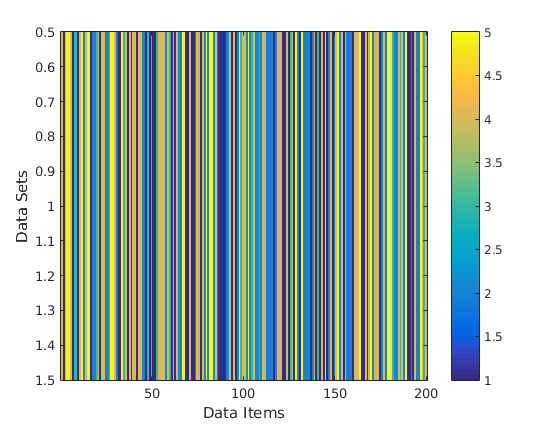
\includegraphics[width = \linewidth]{plots/cluster_smcmdi.png}
\caption{Clustering for Gaussian test data with 5 clusters using SMC\&MDI (no. of clusters restricted to 5)}
\end{figure}

\begin{figure}
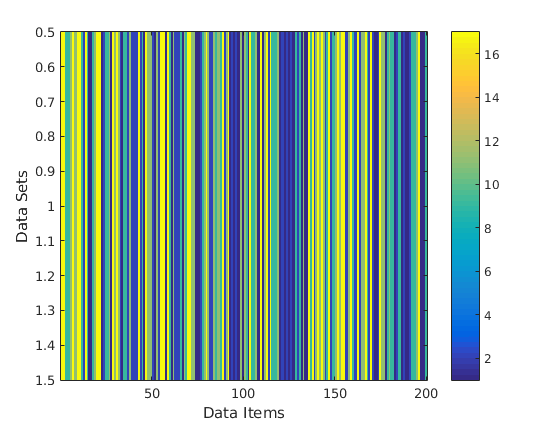
\includegraphics[width = \linewidth]{plots/cluster_mdi.png}
\caption{Clustering for Gaussian test data with 5 clusters using original MDI (no. of clusters restricted to 20)}
\end{figure}
Adjusted Rand Index between the two allocations (below) $<0$. Original MDI code won't run with number of clusters restricted to just 5.
\end{document}

